\chapter{Signal simulation and event selection} 
\label{chap:signalsel}

\section{\ttDM simplified models}
\label{sec:simpmodels}

The dark matter collider signal under investigation is characterized by the production of a top quark pair recoiling against a spin-0 mediator which decays to a pair of dark matter particles, as shown in~\FigureRef{fig:ttDM}. As described in greater detail in Sec, this model predicts the production of dark matter via a scalar (\phi) or pseudoscalar ($a$) mediator, which couples to SM fermions (in this case top quarks) and the Dirac fermion DM particles, with unitary coupling strength (\gq=\gDM=1). 

The most important characteristic of \ttDM models is the \pt of the $\chi\bar{\chi}$ system. This quantity is equivalent to the mediator \pt and is translated to the \ptmiss detector observable in an event. The \ptmiss spectra for the \ttDM models, although dependent on the mediator mass, are expected to peak at higher values than that of the SM \ttbar process, owing to the additional contribution from the $\chi\bar{\chi}$ system. In general, the mediator \pt spectrum broadens with increasing mediator mass, as demonstrated in~\FigureRef{fig:SvPSmedpt}, where the \pt is shown for various scalar and pseudoscalar mediator masses with $M_\chi=1\:\GeV$. It is also the case that at low masses, the pseudoscalar \pt is harder than the scalar \pt of equivalent mediator mass, however the distributions converge to at higher mediator mass. The trend of broadening mediator \pt spectra with increasing mediator mass does not hold in the off-shell regime where the mediator mass is less than twice the DM fermion mass ($2M_\chi > M_\phi$). In the off-shell regime, the \pt of the mediator is not dependent on the mass, and in addition, if the $M_\chi$ is varied for a fixed mediator mass, the \pt distribution is harder for the off-shell production rather than the on-shell. Due to the finite mediator width, in the area near the on/off-shell threshold, the kinematics will contain contributions from both types of production, as seen in~\FigureRef{fig:dmf_medpt2}. 

\begin{figure}
  \begin{center}
    \feynmandiagram[horizontal=c to h]{
      a [particle=\(\bar{t}\)] -- [fermion] b -- [fermion] c -- [fermion] d -- [fermion] e [particle=\(t\)],
      f [particle=\(g\)] -- [gluon] b,
      g [particle=\(g\)] -- [gluon] d,
      c -- [scalar, edge label=\(\phi \slash a\)] h,
      i [particle=\(\bar{\chi}\)] -- [fermion] h -- [fermion] j [particle=\(\chi\)],
      e -- [opacity=0.0001] i,
      a -- [opacity=0.0001] j,
      i -- [opacity=0.0001] j,
%%      f -- [opacity=0.0001] g,
    };
    \caption{The representative diagram of a top quark pair produced in association with a pair of DM particles ($\chi\bar{\chi}$) which decay via an explicit scalar or pseudoscalar mediator coupled to the tops.}
    \label{fig:ttDM}
  \end{center}
\end{figure}

\begin{figure}[htbp!]
  \begin{center}
    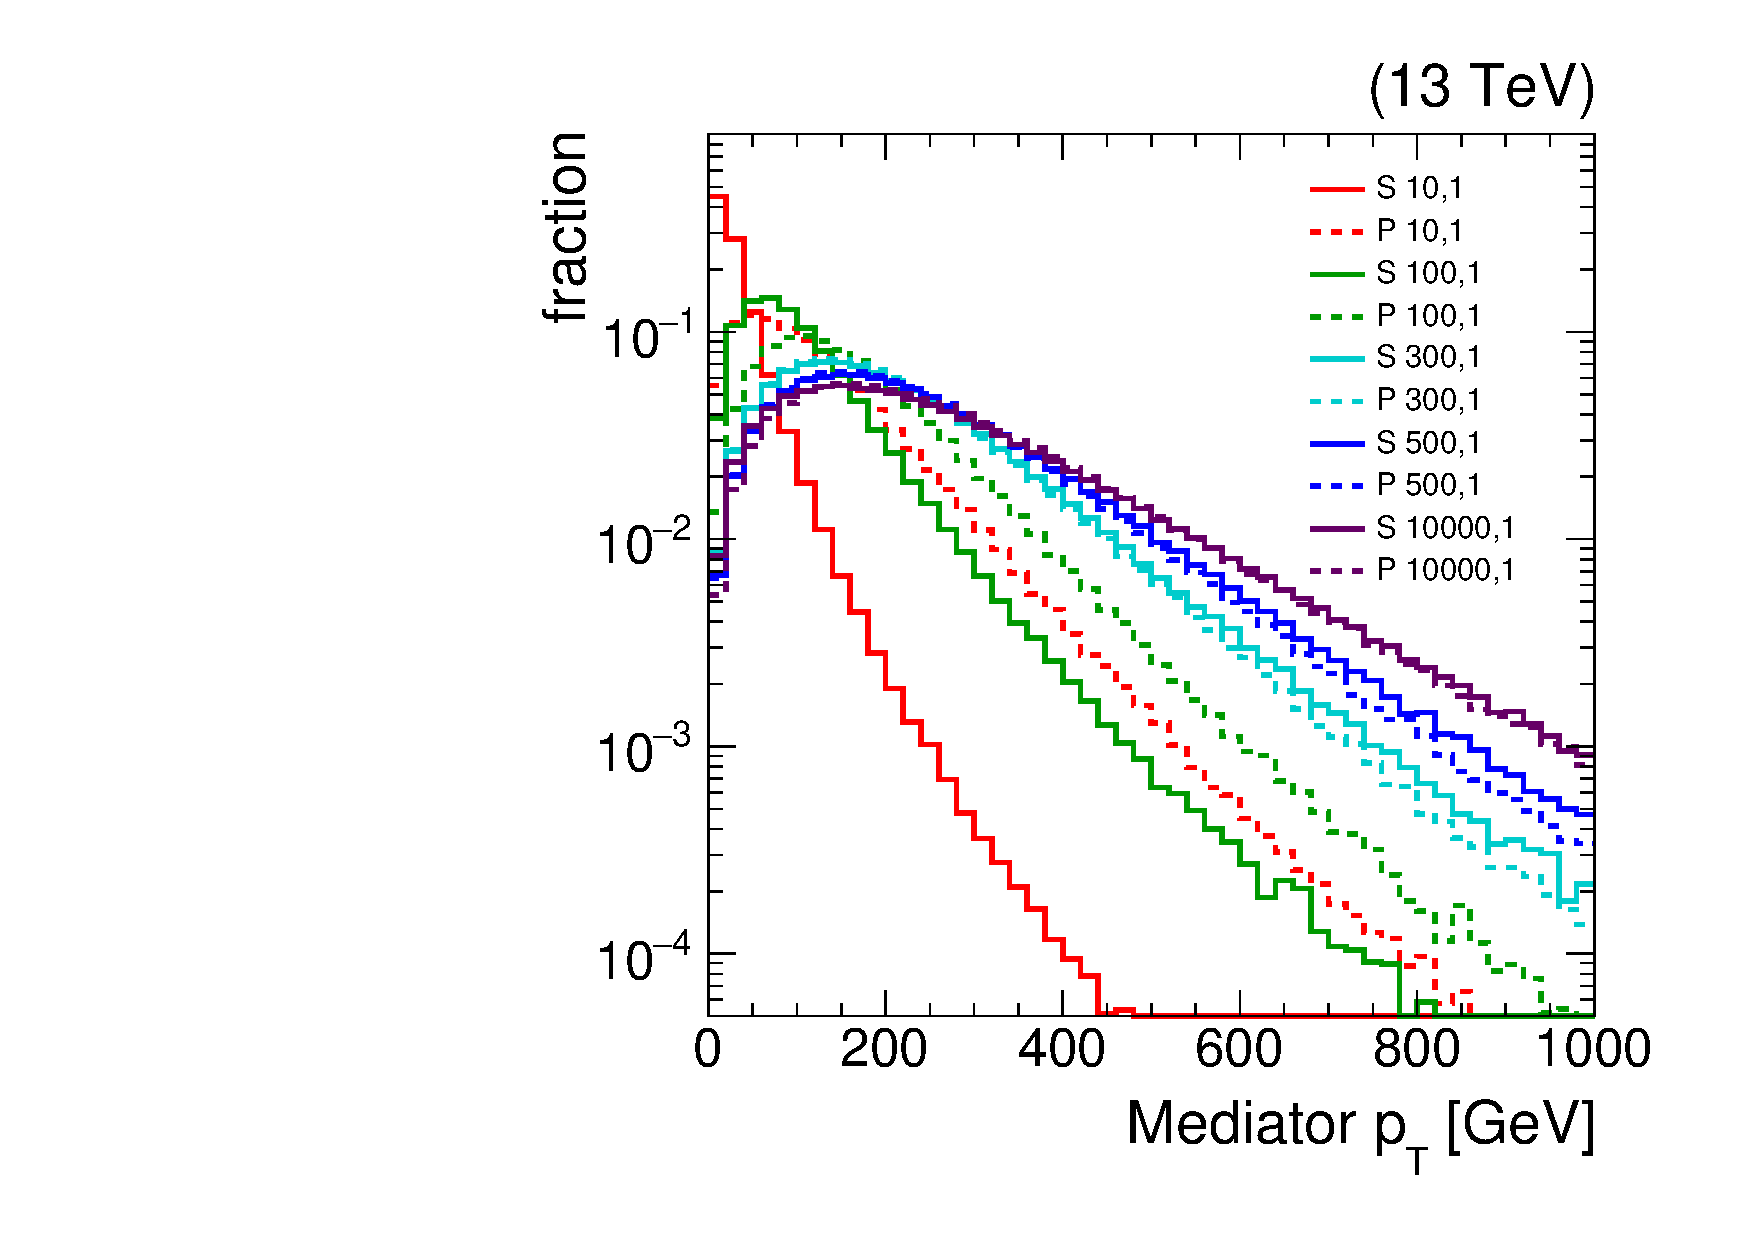
\includegraphics[width=0.48\textwidth]{figs/medptlog.pdf}
    \caption{Generator level \pt distributions for scalar (solid lines) and pseudoscalar (dashed lines) mediators, with $M_\chi=1\:\GeV$, where distributions with the same color have the same mediator mass.}
    \label{fig:SvPSmedpt}
  \end{center}
\end{figure}

\begin{figure}[htbp!]
\begin{center}
  \subfloat[][]{\label{subfig:dmf_off}   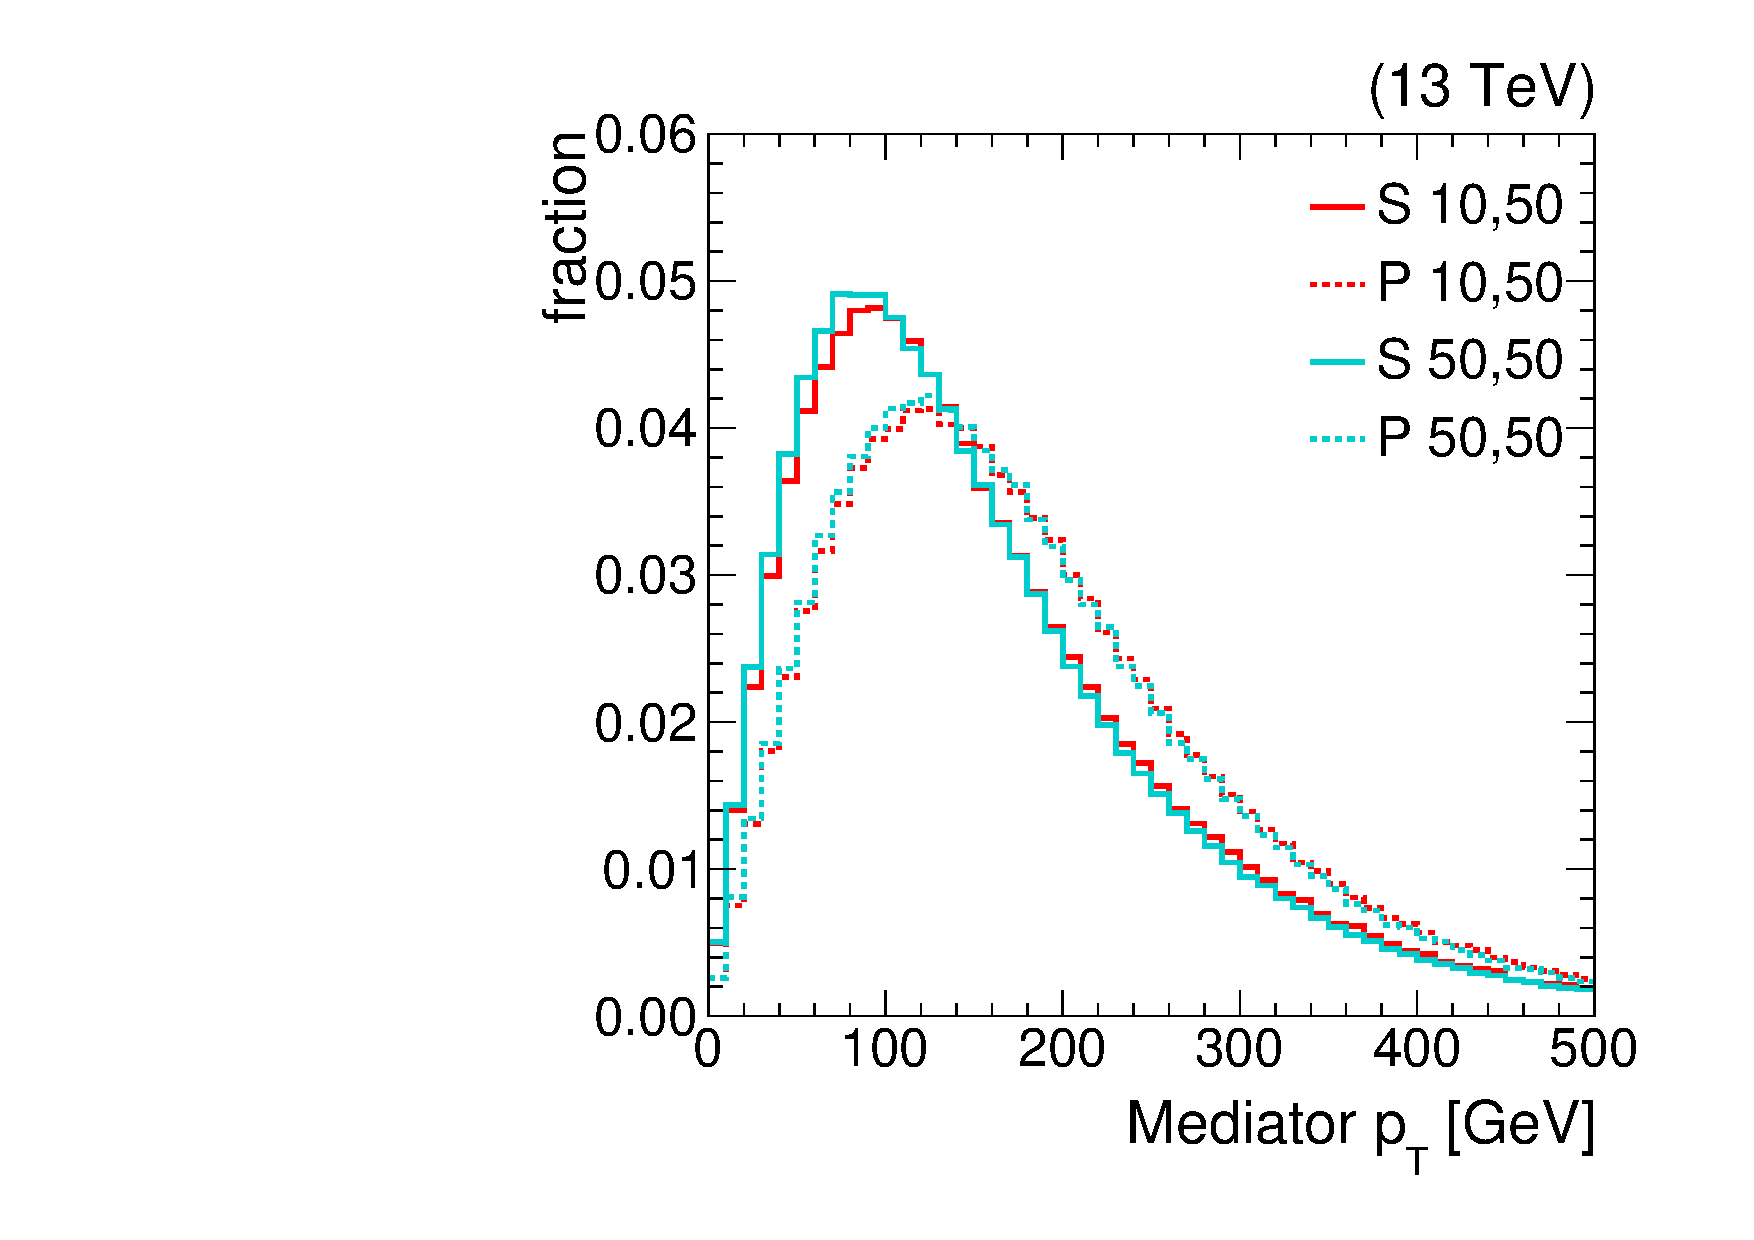
\includegraphics[width=0.48\textwidth]{figs/offshell_medpt.pdf}}
  \subfloat[][]{\label{subfig:dmf_on_off}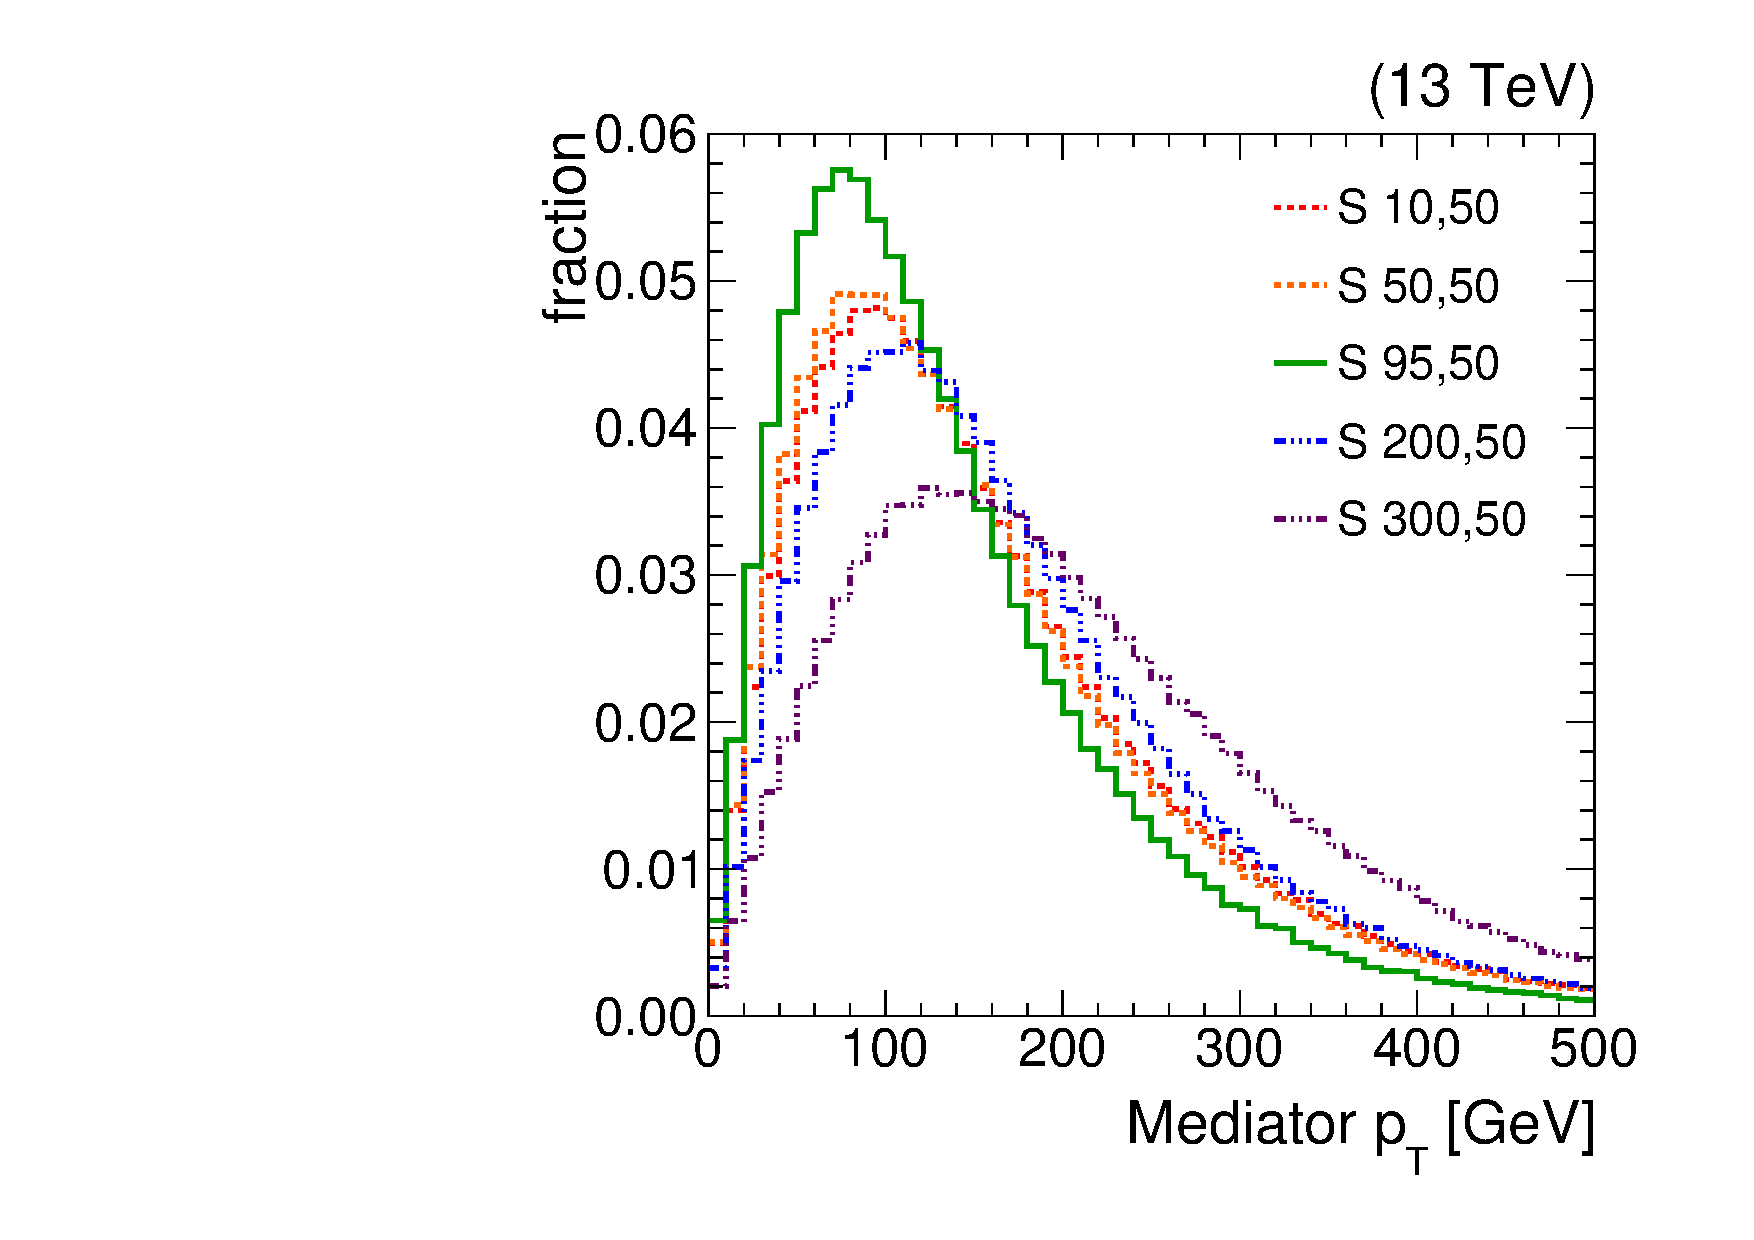
\includegraphics[width=0.48\textwidth]{figs/onshell_vs_offshell_medpt.pdf}}
  \caption{~\protect\subref{subfig:dmf_off} Generator level $\pt$ distributions for off-shell production, with solid lines for scalar and dashed lines for pseudoscalar, and $M_\chi=50\:\GeV$.\protect\subref{subfig:dmf_on_off} Near the on-shell/off-shell threshold (green solid line), the kinematics has contributions from on-shell and off-shell production.}
  \label{fig:dmf_medpt2}
\end{center}
\end{figure}

The \ttDM signals are generated in the dilepton final state at LO accuracy in perturbative QCD using \AMCATNLO \textsc{v2.2.2}~\cite{Alwall:2014hca} with up to one additional jet. The MLM parton-jet matching prescription~\cite{Mangano:2006rw} is used to match jets from the matrix element to the parton shower. The spin correlations in the decays of top quarks are preserved through the use of \MadSpin. The partial width formulae given in ~\cite{PhysRevD.91.055009} are used to calculate the minimum decay widths for the mediators. The calculation assumes that the mediator couples only to SM quarks and the fermion DM particle (\chi), and decays exclusively to a DM pair.  

%%---------------------- Event selection ---------------------- %%
\section{Signal region event selection}
\label{sec:selection}

The objects defined in Sec.~\ref{sec:leps}-\ref{sec:MET} are all employed to target the selection of events consistent with \ttMET where both tops have leptonically decaying W bosons. The selection is as follows,

\begin{itemize}
\item Two ``Tight'' leptons with opposite charge ($ee$ or $e\mu$ or $\mu\mu$) with $\pt>25\:\GeV$ for 
the leading lepton and $\pt>15\:\GeV$ for the trailing lepton,
\item No additional leptons with $\pt>10\:\GeV$ and passing ``Loose'' muon or ``Veto'' electron criter
ia,
\item Two or more jets where at least one jet is b-tagged,
\item $M_{\ell\ell}>20\:\GeV$,
\item $|M_{\ell\ell} - M_Z|>15\:\GeV$ for $ee$ and $\mu\mu$ events,
\item $\ptmiss>50\:\GeV$,
\end{itemize}

Dilepton candidate events with an invariant mass $M_{\ell\ell}<20\:\GeV$ are removed in order to suppress any backgrounds from low-mass Drell-Yan processes, as well as any contributions from heavy-flavor resonances. The requirement for events in the same flavor ($ee$ and $\mu\mu$) channel to have an invariant mass $\pm15\:\GeV$ away from the Z boson pole mass is also used to reject $Z(\ell\ell)$ background events. The moderate requirement of \ptmiss$>50\:\GeV$ aims to further suppress contamination from DY events in the same flavor channel.

\subsection{The \mttll variable}
\label{subsec:mt2ll}

Along with categorization according to lepton flavor (same or opposite), events are also categorized based on the stransverse mass quantity, \mttll, defined as,

\begin{equation}
  M_{\text{T2}}^{\ell\ell} = \min_{\vec{p}^{\text{miss}}_{\text{T1}}+\vec{p}^{\text{miss}}_{\text{T2}}=\vec{p}^{\text{miss}}_{\text{T}}}\left(\max\left[M_{\text{T}}\left(\vec{p}^{\ell_1}_{\text{T}},\vec{p}^{\text{miss}}_{\text{T1}}\right),\:M_{\text{T}}\left(\vec{p}^{\ell_2}_{\text{T}},\vec{p}^{\text{miss}}_{\text{T2}}\right)\right]\right),
  \label{eq:mt2ll}
\end{equation}

\mttll is partially motivated from the transverse mass, denoted $M_{\text{T}}\left(\vec{p}^{\ell}_{\text{T}},\vec{p}^{\text{miss}}_{\text{T}}\right)$ in Eq.~\ref{eq:mt2ll}, where the most notable use of \mt is in the measurement of the $W$ boson mass in the $W\rightarrow\ell\nu$ decay mode. The transverse mass, defined in the context of a leptonic $W$ boson decay, is as follows,

\begin{equation}
  M_{\text{T}} = \sqrt{M_{\ell}^{2} + M_{\nu}^{2} + 2(E_{\text{T}}^{\ell}E_{\text{T}}^{\nu} - \vec{p}_{\text{T}}^{\ell}\cdot\vec{p}_{\text{T}}^{\nu})}
\end{equation}

where $M_{\ell}$ and $M_{\nu}$ are the masses of the lepton and neutrino, respectively, and $\vec{p}\
_{\text{T}}^{\ell}$ and $\vec{p}_{\text{T}}^{\nu}$ are their transverse momenta. $E_{\text{T}}^{\ell}$ and $E_{\text{T}}^{\nu}$ denote their transverse energies. 

The utility of $M_{\text{T}}$ is best for cases wherein one missing particle is expected (i.e. the neutrino in the leptonic $W$ decay). However, once more than one missing particle is expected in an event, it is no longer possible to calculate the \mt since the \pt of an individual missing particle cannot be resolved. Recalling that \ttDM production and decay follows this route:

\begin{equation}
pp \rightarrow t\bar{t} + \phi \rightarrow W^{+} b + W^{-} \bar{b} + \XX \rightarrow \ell^{+} \nu b + \ell^{-} \bar{\nu} \bar{b} + \XX,
\end{equation}

a signal event is expected to contain four particles that leave their signature in the detector collectively as \ptmiss, namely the $\nu,\:\bar{\nu},\:\chi,\:\bar{\chi}$. Similarly, in the case of the SM \ttll process, the two lepton neutrinos are the sole contributors to the total \ptvecmiss, and as postulated by the authors in~\cite{Lester:1999tx}, if the $\vec{\pt}^{\nu}$ and $\vec{\pt}^{\bar{\nu}}$ were obtainable, the maximum \mt value is bounded from above by the $W$ boson mass such that,

\begin{equation}
  M_{W}^{2} \geq \max{\{M_{\text{T}}^{2}\left(\vec{p}^{\ell^{+}}_{\text{T}}, \vec{p}^{\nu}_{\text{T}}\right), M_{\text{T}}^{2}\left(\vec{p}^{\ell^{-}}_{\text{T}}, \vec{p}^{\bar{\nu}}_{\text{T}}\right)\}}.
\end{equation} 

The partitioning of the \ptvecmiss is however unknown, since neither the energy nor direction of either neutrino four-vector can be resolved, so the best that can be assumed is, 

\begin{equation}
  M_{W} \geq M_{\text{T2}}^{\ell\ell} = \min_{\vec{p}^{\text{miss}}_{\text{T1}}+\vec{p}^{\text{miss}}_{\text{T2}}=\vec{p}^{\text{miss}}_{\text{T}}}\left(\max\left\{M_{\text{T}}\left(\vec{p}^{\ell_1}_{\text{T}},\vec{p}^{\text{miss}}_{\text{T1}}\right),\:M_{\text{T}}\left(\vec{p}^{\ell_2}_{\text{T}},\vec{p}^{\text{miss}}_{\text{T2}}\right)\right\}\right).
\label{eq:mt2ll_2}
\end{equation}

The minimization in Eq.~\ref{eq:mt2ll_2} occurs over all the possible two-way partitions of \ptvecmiss in the event. For the case of the SM \ttll background, a kinematic endpoint in the \mttll distribution, shown in~\FigureRef{fig:mt2ll}, occurs at the $W$ boson pole mass. With this in mind, two signal regions are formed using the \mttll variable, where events with \mttll$>110\:\GeV$ comprise the high signal purity region, since the signal is not expected to be contained in the region below the $M_W$ as is the case for the SM \ttll background. The low signal purity category is formed by the remaining events, for which \mttll$<110\:\GeV$.

\begin{figure}
  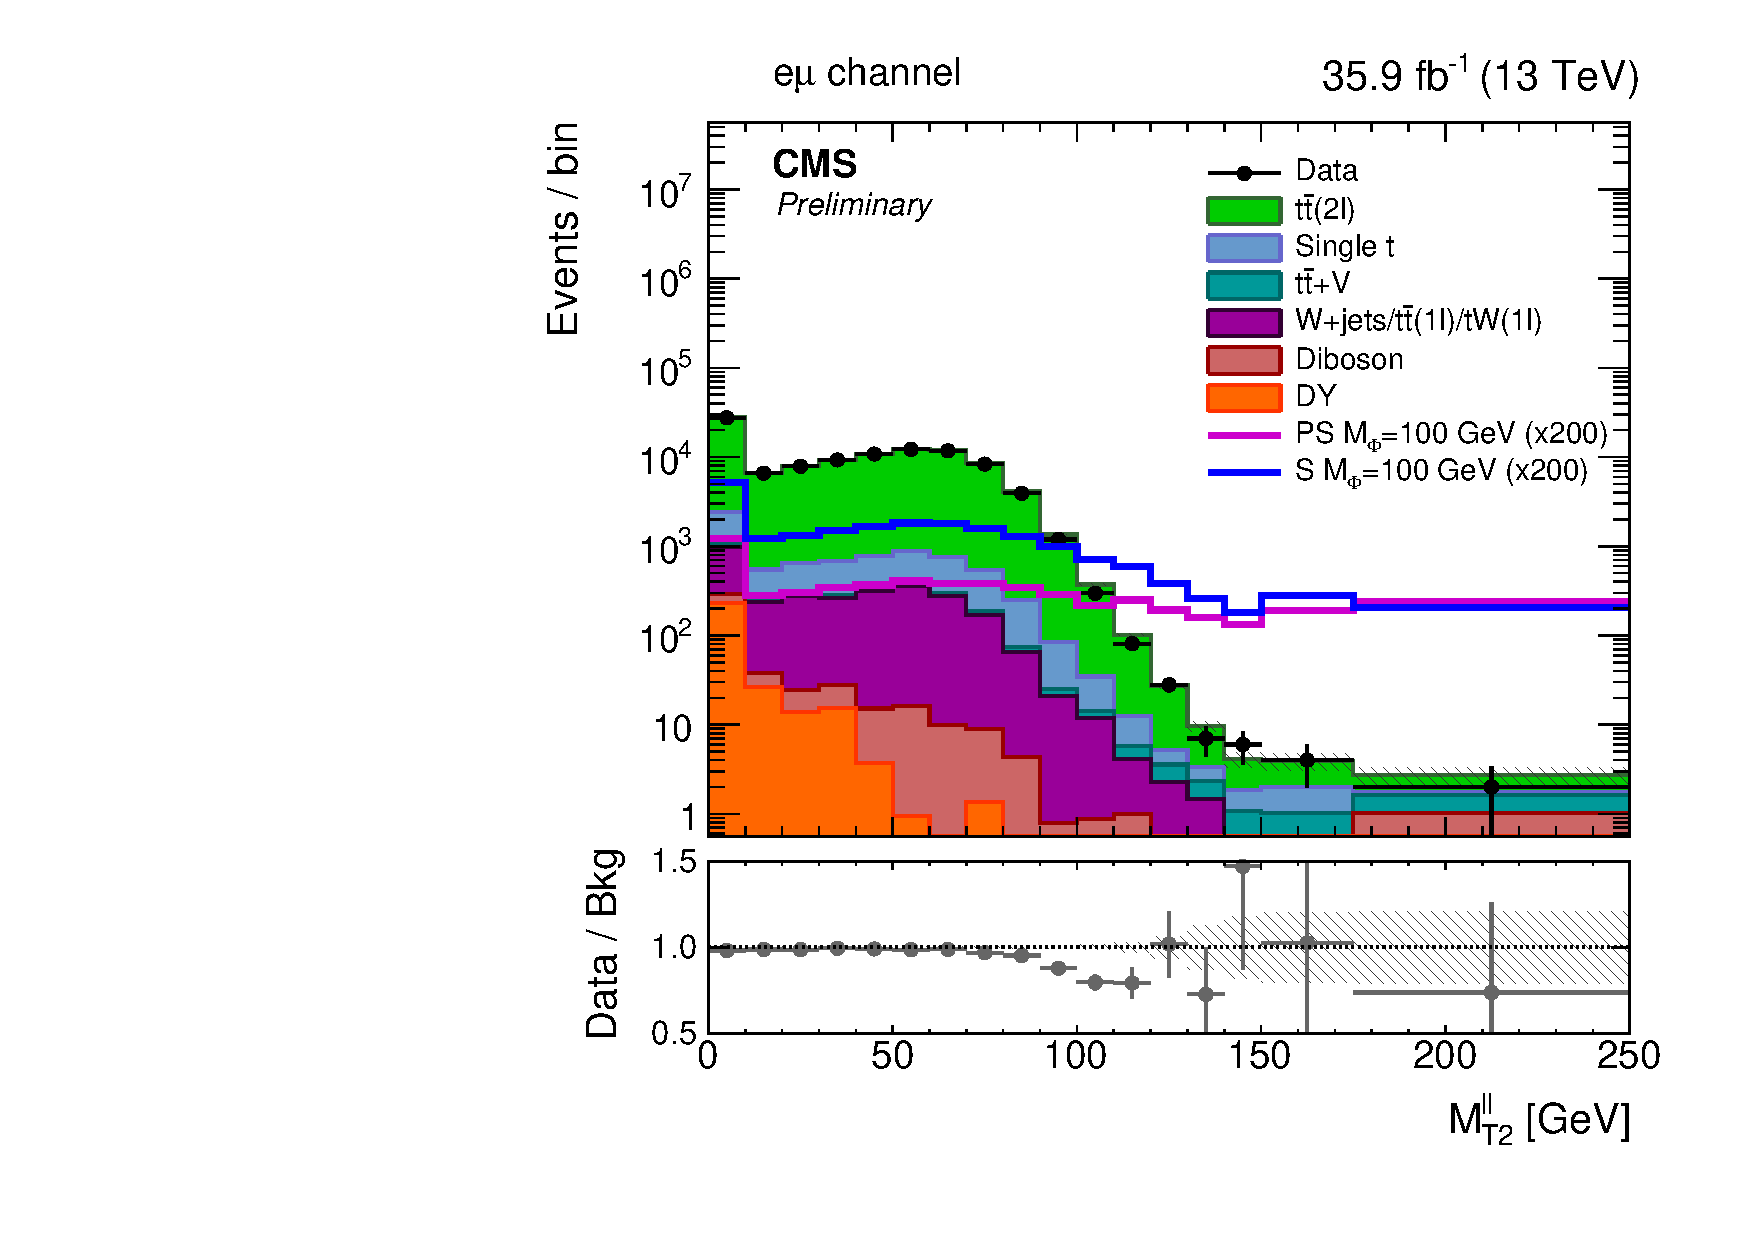
\includegraphics[width=0.6\textwidth]{figs/mt2log_em.pdf}
  \caption{The \mttll distribution in data and simulation for events passing selection requirements for the $e\mu$ channel. The distribution of two example signals (scalar and pseudoscalar mediator, $M_{\phi/a} = 100\:\GeV$) with $M_{\chi}=1\:\GeV$ is scaled up by a factor of 200. The last bin includes overflow. Uncertainties are statistical only.}
  \label{fig:mt2ll}
\end{figure}
